\section{Structured Indoor Modeling} \label{section:room}

This section presents our implementation of the structured modeling
framework for the indoor scenes.
%The full structure grammar is provided in Fig.~\ref{fig:graph_grammar}
%and the supplementary material.
%
After explaining our input data, we will show the overall modeling framework and individual
structure grammar rules with the corresponding reconstruction
algorithms.

\subsection{Input data}
\textcolor{red}{Panorama RGBD images are acquired by a camera and a depth sensor mounted on a motorized tripod. It takes a couple of minutes to acquire a single panorama RGBD image, and they are aligned by the ICP algorithm after rough manual initialization.} Several filtering techniques are used to pre-process data, 
%Our input is a set of calibrated RGBD panoramas.
%%from the color and depth sensors mounted on a motorized tripod.
%Standard procedures are used to pre-process data, 
whose details are referred to the supplementary material. There are a few things worth noting here.
% A standard ICP~\cite{besl-mckay-pami-1992} algorithm with manual
% initialization registers the depth data. The alignment between the color
% and depth sensors are obtained by calibration. A surface normal is
% estimated for each 3D point by a local plane fitting. Note that we know
% the unit of the depth values from the depth sensors.
% %, while SfM and MVS reconstructions are usually scale ambiguous.
% %\mysubsubsection{Manhattan frame extraction}
% %The input coordinate frame may not be aligned with the dominant scene
% %directions.
First, we extract the Manhattan directions from the input point
clouds~\cite{ManhattanWorldStereo}, and transform the data into the
Manhattan coordinate frame with the Z-axis pointing to the ``up
direction''. Second,
%
% \mysubsubsection{Noise removal} 3D points suffer from gross errors due
% to reflective and transparent materials.
% % abundant in indoorscenes.
% %(\eg windows, glass cups, mirrors, and metalic appliances).
% A depth measurement comes with an intensity reading.
% %we found that a simple thresholding is effective in removing noisy 3D
% %points. More concretely,
% For each depth image, we compute their mean $\mu_i$ and the standard
% deviation $\sigma_i$, and discard points whose intensities are below
% $\mu_i - 2 \sigma_i$.
%
%\mysubsubsection{Point and free-space evidences}
%Like most existing work,
the point $P(v)$ and the free-space $F(v)$ evidences are calculated for
each voxel $v$.
% We firstly compute the bounding box of the entire point cloud, and
We discretize the bounding box of the 3D points, where the voxel size is
set to $0.012\mbox{m}$.
$P(v)$ counts the number of 3D points inside. $F(v)$ counts how many
times the voxel is intersected with visible rays. $P(v)$ and $F(v)$ are
normalized so that their greatest value becomes $1$, respectively.

% then divide the box into sub-voxels whose size is
% $w\times h \times d$. Then each point is projected onto one of
% sub-voxels. For each voxel cell, we compute two kinds of 3D evidence in
% the same manner with existing works~\cite{}; the point evidence ($E^P\in
% \mathcal{R}^{h\times w\times d}$) that collects the number of points in
% each cell, and the free-space evidence ($E^F\in \mathcal{R}^{h\times
% w\times d}$) that collects the number of times the cell is intersected
% by rays connecting a point to its corresponding camera center.

% In addition, we define the {\it 2D} point/free-space evidences
% $\tilde{E}^F, \tilde{E}^P\in \mathcal{R}^{h\times w}$ on the $X-Y$
% coordinate system, which counts how many cells are occupied in $E^P$ and
% $E^F$ with regard to $Z$-axis \ie, the highest value is given when the
% cells have values from $z=0$ to $z=d-1$.


\subsection{Modeling pipeline}

The structured modeling repeats applying grammar rules whose
pre-conditions are satisfied, until no rules can be applied.  The
structure graph is initialized with a scene node, and the room
segmentation is the only applicable rule initially.  In practice, the
following two guidance are also used to control the rule applications:
First, the wall detail reconstruction is applicable only after the
system terminates with the remaining rules.  Without the restriction,
the wall details might be reconstructed for a room, but the room could
be later merged and removed, yielding wasted computations. Second,
whenever a new room node is created, the room reconstruction rule is
triggered, as this is the only applicable rule for a newly generated
room node.
% A room node would be deleted if the room
% reconstruction fails, and we would like to conduct the test as soon as
% possible.
This algorithm is not guaranteed to terminate, as it may iterate
creating and removing rooms. However, our experiments show that the
algorithm terminates efficiently in all our examples.


\subsection{Indoor structure grammar}

Our indoor reconstruction process is governed by the eight structure
grammar rules illustrated in Figure~\ref{fig:graph_grammar}.
% We here focus our description to the five key rules. The remaining three
% rules (room addition, room merging, and object reconstruction) are
% relatively simple and their description is given in the supplementary
% material.
Due to the space limitation, we restrict our description to the major
rules in this paper. The remaining three rules together with minor
algorithmic details are given in the supplementary material. The actual progress of the graph construction is illustrated in~\Fref{fig:graph}.
%are minor, and the details are given in the supplementary material.
\begin{figure*}[tb]
\begin{center}
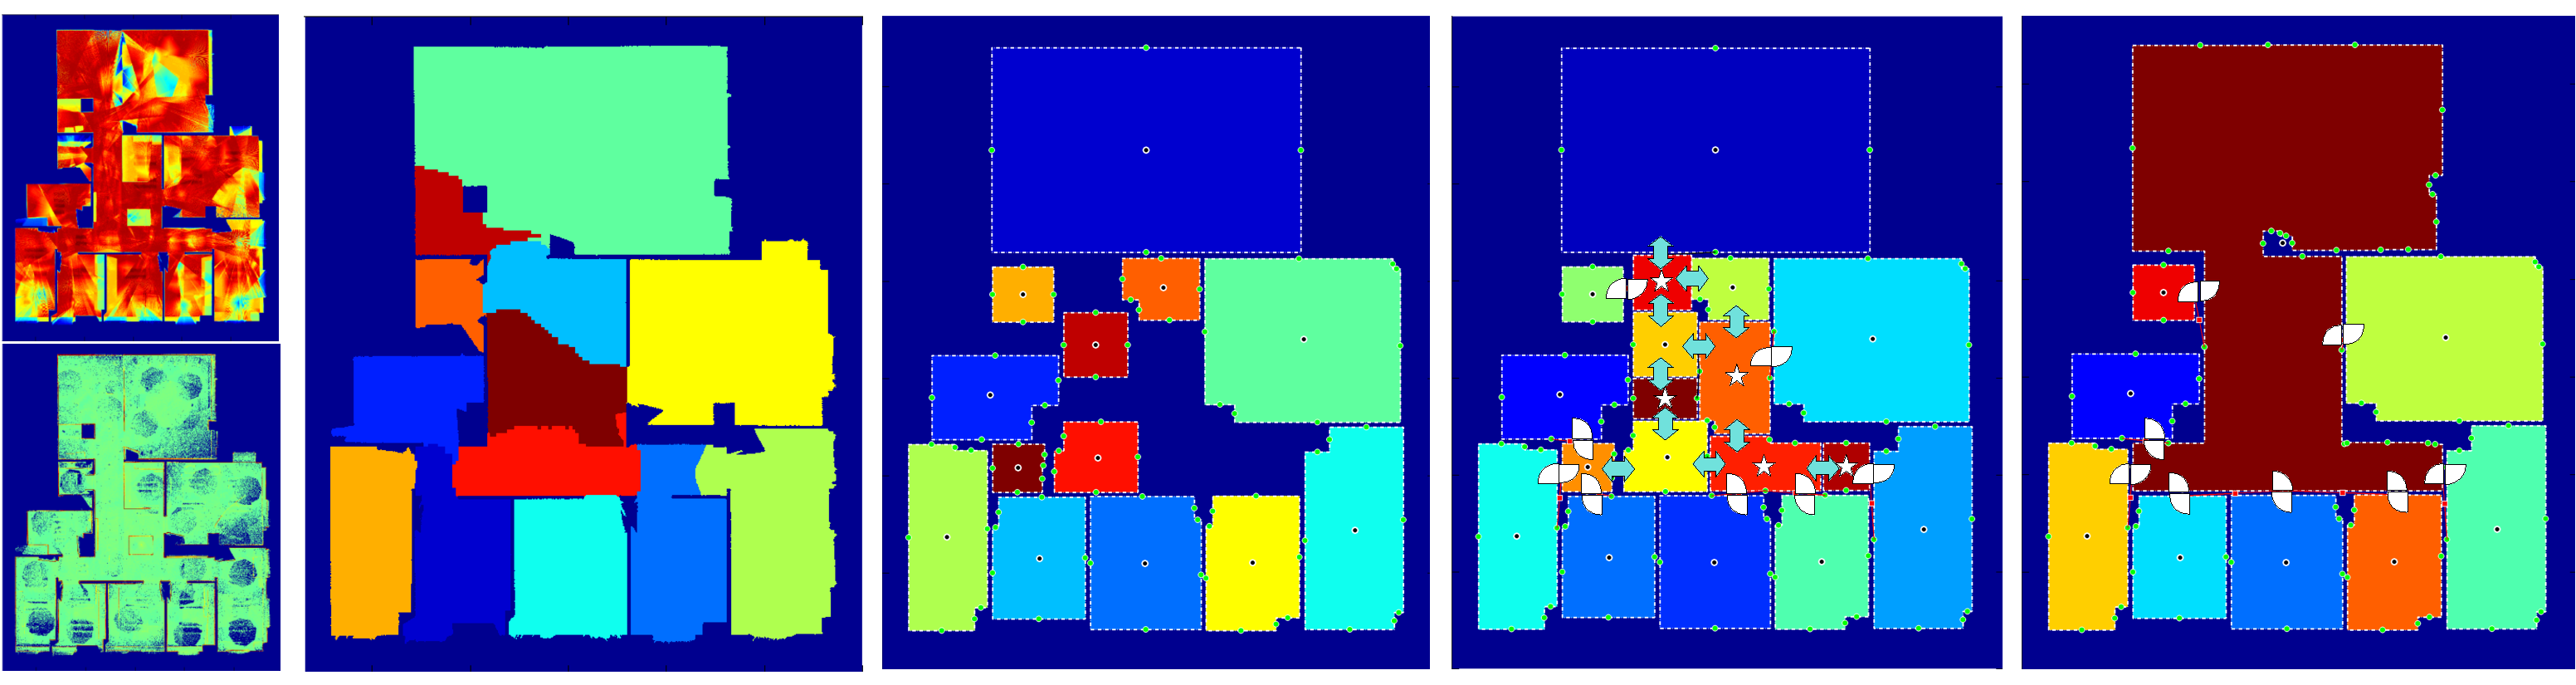
\includegraphics[width=160mm]{../figures/graph2.pdf}
\end{center}
\caption{Structured graph representation and its construction. Starting
from the generation of the free-space end point evidence (left), we
perform the room-segmentation and reconstruction (2-nd and 3-rd column).
More rooms are added and the room connection types are classified (4-th
column). The white icon represents the ``door'', while the blue icon
 represents the ``merge'' classification.
 We finally get the structured graph representation as
shown in the last column. Here we only show the spatial relationships
for simplicity. }
% as we have described in the previous sections.
   \label{fig:graph}
 \vspace{-0.325cm}
\end{figure*}



\mysubsubsection{Room segmentation} The rule obtains the initial room
segmentation on the XY-plane. Room boundaries are often ambiguous, and
full 3D analysis will be conducted in future rules to refine the
segmentation. The rule takes a scene (pre-condition) and creates
multiple rooms (transformation).
%
%
%
% This is the first one to be applied in our modeling pipeline.
%
% To avoid primitive detection, which is the major failure mode of
% existing methods~\cite{MWS,museum,sinha?},
%The framework globally analyzes an entire indoor space on an XY-plane
%(i.e., a top-down view).
\begin{figure}[!t]
\begin{center}
%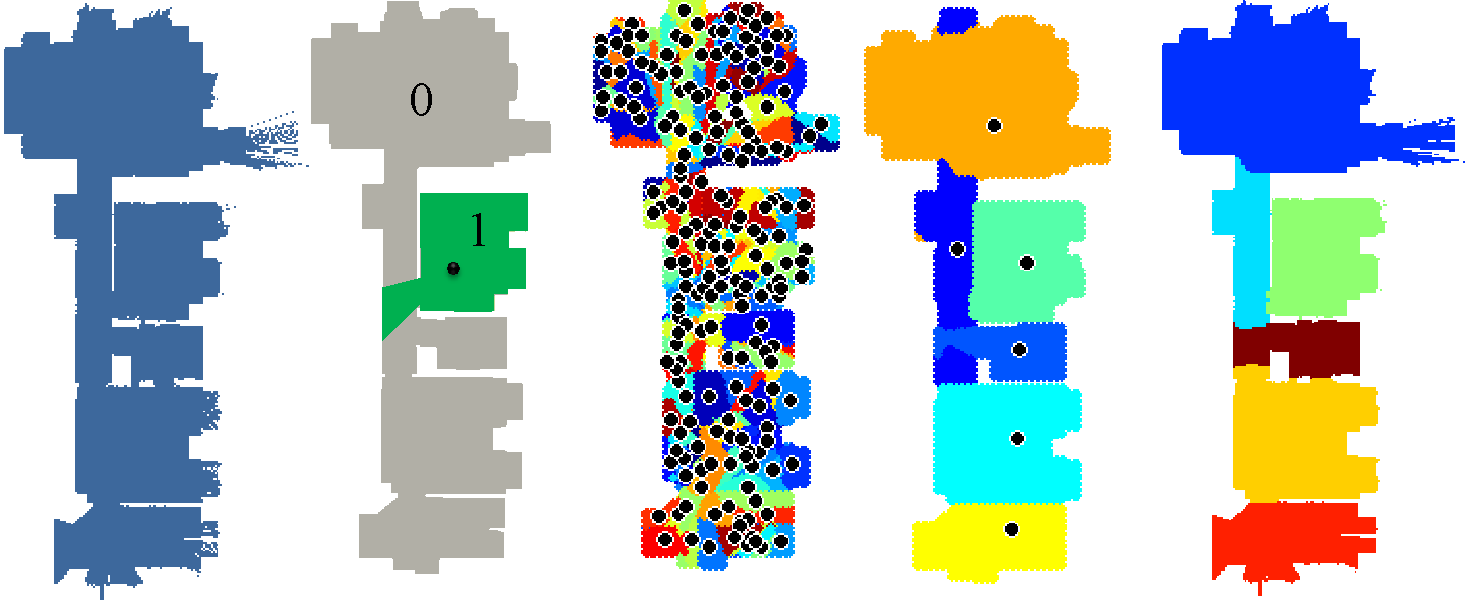
\includegraphics[width=85mm]{../figures/k-medoids.pdf}
 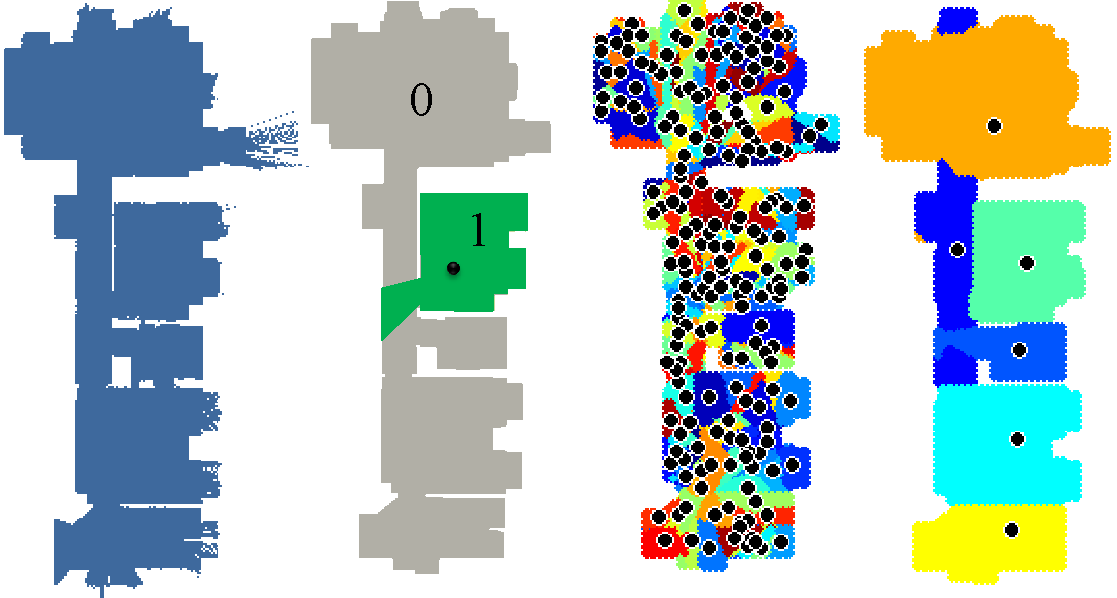
\includegraphics[width=75mm]{../figures/k-medoids2.pdf}
\end{center}
\caption{Room segmentation. From left to right: 1) The domain is
 obtained by thresholding the free-space evidence. 2) The refined
 domain, and the visibility information at a pixel. 3) Initial 200 clusters
 of the k-medoids algorithm. 4) The final clusters. A pixel in the
 domain is colored based on the nearest cluster center.
%  5) 
%  The illustration of the room segmentation. (a) we binarize
% the free-space evidence by 0 or more than zero, and cut-off some small
% fragments as shown in (b). Visibility features are computed between interior samples
% and boundaries (in this example the boundary pixels inside the green region could be visible from the black dot). Based on these features, we perform k-medoids clustering
% algorithm from $200$ cluster centers (c) to the convergence (d) and then
% labels of sparse samples are propagated to the entire free-space
 % (e). }
 }
\label{fig:k-medoids}
 \vspace{-0.325cm}
\end{figure}


The room segmentation is formulated as a clustering problem.
%on the XY-plane (See Fig.~\ref{fig:k-medoids}).
%Let $F_{2D}(p)$ denote the free-space evidence that is summed along the
%Z-axis, where $p$ is a discretized 2D pixel on the XY plane.
First, the domain $\Psi$ is initialized by the pixels, where the sum of
the free-space evidences along the Z-axis is non-zero.
%The following heuristic is used to refine $\Psi$:
$\Psi$ is then refined by removing pixels, whose distances to the
closest boundary of $\Psi$ along the X or Y axes are less than
$0.8$m. This heuristic is effective in removing thin erroneous regions
near windows. Second, the k-medoids algorithm is used to cluster
subsampled pixels (at every $100$mm along X and Y) in $\Psi$.
%
% with a subsampling ratio of 100 \yasu{how do you subsample for
% k-medoids?}{\ikehata{For interior samples, I computed the grid whose
% margin is $100$ mm and took samples from every corner of the grid that
% are in the free-space evidence. And for boundary samples, I take one
% sample every $100$ mm on the contour}}.
%
The distance metric for clustering is based on a ``binary visibility
vector'' $V(p)$ for each pixel $p$.
%The dimension of $V(p)$ is equal to the number of pixels at the boundary
%of $\Psi$.
%
%After discretizing the boundary of $\Psi$ to a finite number of points,
%
%For each pixel $p \in \Psi$, we calculate a ``binary visibility vector''
%$V(p)$,
The $i_{\mbox{th}}$ element $V_i(p)$ of the vector is 1, if $p$ is
visible from the $i_{\mbox{th}}$ boundary pixel through $\Psi$.
Intuitively, the vector $V(p)$ stores which of the scene boundary is
visible from $p$.
The distance of the two pixels $p$ and $q$ is given by the hamming
distance of $V(p)$ and $V(q)$ divided by $\sum_i V_i(p) \sum_i
V_i(q)$. The division converts the distance range to $[0, 1]$.
% makes sure that the distance is at most $1$.
%Intuitively, two pixels belong to the same room, if the common visible
%surface is great.
%two pixels with a lot of common visible surfaces 
%the more common visible surfaces, the more likely two
%pixels belong to the same room.
%this metric measures the amount of common visible surfaces.
% this measures the amount of overlap of visible region boundaries.
%
Starting from $200$ clusters, we repeat the k-medoids
algorithm and the cluster merging, where two adjacent clusters are
merged if the distance between their centers is less than 0.4.
%\ikehata{it seems that this part lacks the unexplained region extraction
%but should be included as the ''post-condition'' since we judge the
%segmantation failes where many ''unexplained" regions and want to add
%room nodes to them.}
%\yasu{No, unexplained region is room-addition rule. pre-condition of that
%rule handles that.}
Lastly, the segmentation results are propagated to all the pixels in $\Psi$
by the nearest neighbor.
% Once the sample is extracted and the visibility feature vectors are
% computed, we cluster $S_{\tilde{E}^F}$ using standard k-medoids
% algorithm based on the visibility features. K-medoids clustering is a
% partitioning algorithm, which attempts to minimize the SSE (Sum of
% Squared Error) between samples and cluster centers. Instead of taking
% the mean values a cluster center, K-mediods algorithm represent the
% cluster center by one of samples in a cluster. We should note that the
% visibility feature is a binary vector (\ie, each element is $1$
% (visible) or $0$ (not visible)), therefore the distance between two
% vectors efficiently computed by a hamming distance. However, the
% standard hamming distance computation is insufficient for the room
% segmentation problem since when the room size is small, the number of
% boundary pixels that explain the room is very small. For normalizing the
% contribution of the boundary pixels in a clustering, we normalize the
% visibility feature by the number of non-zero elements in each vector and
% using the weighted hamming distance for the distance computation.

% As a actual procedure, we firstly fix the initial number of clusters by
% a somewhat large number (\eg, 100), then merge two clusters when the
% distance between two cluster centers are less than a threshold
% ($TH_2$). Once the labels are assigned to sub-samples, we estimate the
% labels of other pixels that meet $\textbf{E}^F_p>0$ and $p \notin
% S_{\tilde{E}^F}$ by assigning labels of nearest neighbor pixels w.r.t
% the geodesic distance on the binary free-space evidence. Finally we
% assign the room node to each cluster with index list of the pixels.

% The resulting room segmentation is not perfect. Especially the boundary
% between two rooms is quite in accurate and often gives wrong number of
% rooms. Therefore, we use this result as a initial estimate of the room
% segmentation and update the result through the resulting wall and door
% elements reconstruction.

\mysubsubsection{Room reconstruction} This rule takes a room that has
not been reconstructed yet, that is, a room node without any edge except
for the incoming directed one (pre-condition). A room outline in a top-down
view is reconstructed as a 1D polygon, which is extruded to the
estimated floor and ceiling heights to generate a 3D model. This rule
generates a floor, a ceiling and a chain of wall nodes (transformation).
%
% \ikehata{Actually, I do not discard the reconstruction results when
% firstly performing the shortest path reconstruction since each clusters
% are always satifactry large. But when performing unexplained region
% extraction, I discard the room proposals when (a) the core-freespace
% size is less than 0.05*mean(otherroomsize) and the
% sum(pointevidence(0-1))/sum(freespace(0-1)) is less than 0.5}

A room outline is generally piecewise planar and consists of a very few
number of vertices. We employ the shortest-path based algorithm that is
optimized to produce such a shape~\cite{Cabral2014}. There is one
modification worth noting. The original algorithm requires the addition
of ``anchor'' points to overcome the shrinkage bias.
%(\eg thin walls at the room boundaries).
This is essential in their work, as they reconstruct an entire scene
(i.e., multiple rooms) with a single shortest-path algorithm.
%
In this work, the algorithm is applied to each segmented
room individually, and does not require anchor points.
% We have also made a few minor improvements over the original algorithm,
% and refer the details to the supplementary material.
%
%However, they are not the core contribution of this paper and referred
%to the supplementary material.
The floor and ceiling heights are estimated by horizontal plane fitting
via RANSAC, 
%fitting horizontal planes
%to the 3D points in a room by RANSAC,
below and above the average camera height, respectively.
% \yasu{A little strange
% here. Do you just extract 2 dominant horizontal planes by
% RANSAC?}\ikehata{I firstly split the points into two (a) lower than
% camera center and (b) higher than the camera center and then simply
% perform the RANSAC-based plane fitting whose normal is exactly
% perpendicular to the X-Y coordinate.}

% Once the room, wall, door elements are reconstruced except their
% geometry, we compute the ceil and floor heights using a point cloud that
% can be projected onto the supported room pixels on the 2D voxel grid. We
% simply perform the RANSAC-based plane fitting with a constraint that the
% surface normal of the plane is parallel to the Manhattan $X-Y$
% coordinate.





% Given room elements $\textbf{R}$, we aim to reconstruct the wall
% elements $\textbf{W}$ that are the adjoined piecewise 2-D paths. For
% instance, one room that has four walls could be decomposed into the four
% piece-wise planar paths that is exactly lying on the wall and the
% start-end paths are connected with each other, which is very important
% property of preserving the {\it manifold-ness} of the wall structure. We
% can also see these paths as simplified geometry of the walls of a room
% since if we pump-up the wall path to the ceiling height, we can get the
% piece-wise planar room geometry.

% We tackle this problem based on the existing floorplan reconstruction
% technique based on the shortest path
% algorithm~\cite{Cabral2014}. However, we cannot straight forwardly
% perform their method since we should consider the existence of other
% rooms (and their walls) while the room structure has not been considered
% in~\cite{Cabral2014}.

% For each room, we generate a binary mask ($B_i \in \mathcal{L}^{h \times
% w}$) where the value at a cell included in the pixel index list of
% $\textbf{R}_i$ is one, and other wise zero. Then we perform the
% morphological closing operations as described in the previous
% section. Using this mask, we extract three information for solving the
% shortest path problem; (a) the local wall evidence, (b) the core
% free-space, and (c) the start-end line.

% Firstly we generate the local wall evidence for $i$-th room ($\tilde{E}^W_i$) as
% \begin{equation}
% \tilde{E}^W_i = \begin{cases}
% 1 & (B_i=1)\;{\rm and}\;(\tilde{E}^W=1).\\
% 0 & (otherwise).
% \end{cases}
% \end{equation}
% Then, we compute the core free-space of $i$-th room ($\Omega$) by solving following equation, 
% \begin{equation}
% \min_{\Omega \in RectSet_i} max(H_{\Omega}, W_{\Omega}) + \gamma H_{\Omega}W_{\Omega}.
% \end{equation}
% where ${RectSet_i}$ is a collection of rectangles that are completely included in the non-zero regions of $B_i$ and $H_\Omega$ and $W_\Omega$ are height and width of a rectangle proposal. This core-frespace evidence quantifies the reasonable observation that the room shape is generally convex except for the details on the wall such as walls, pillows, and some planar structure (\eg, kitchen counter).


% Once we compute the local wall evidence and core-freespace, we compute the start/end line that constrains the shortest path algorithm. In the similar manner with~\cite{Cabral2014}, a start/end-line is denoted as an array of cells: $\{c_1,\cdots,c_{j-1},\cdots,c_j,c_{j+1},\cdots,c_n\}$ and start and end cell is described as $c_s, c_e$, where $c_1$ touches the core free-space, $c_n$ touches the domain boundary, and $c_j$ is the cell containing the start/end point. Then, we find the start-end line by minimizing the following function,
% \begin{eqnarray}
% \tilde{E}_i^W(c_s)+\tilde{E}_i^W(c_e)+\tilde{E}_i^W(c_j)\nonumber\\
% -\sum_{k=1}^{n}\tilde{E}_i^W(c_{j+k}).
% \end{eqnarray}

% Given three information (a) the local wall evidence, (b) the core free-space, and (c) the start-end line, then we reconstruct the shortest path ($P_{wall}$) that represent the wall elements of a room element $\textbf{R}_i$ by solving following equations,
% \begin{equation}
% \min_{P\in P_{c_s\rightarrow c_e}} \sum_{k=1}^{|P|} e_{\rho_k}, \label{eq:shortestpath}
% \end{equation}
% where $P_{c_s\rightarrow c_e}$ is all possible paths that connect the start cell $c_s$ and the end cell $c_e$ that consist of vertical or horizontal edges ($\rho$) in the 2D voxel grids. And,  $e_{\rho}$ is a edge cost that is defined as,
% \begin{eqnarray}
% e_{\rho} = \frac{1}{1+\beta}\sum_{k=1}^{|\rho|}{\left(1-\tilde{E}^W_i(c_k)+ \beta \tilde{E}^F(c_k)\right)}\nonumber\\
% +\omega + F_{penalty}(\rho),\label{eq:edgecost}
% \end{eqnarray}
% where $\beta$ is a weight that balances the contribution the free-space
% evidence and wall evidence and $c_k$ is a cell that is included in the
% path segment $\rho$. In \Eref{eq:edgecost}, the first term penalizes
% going though low wall-evidence cells and high free-space evidence
% cells. And second therm is a constant mode-complexity penalty, which
% biases our solution towards paths with less edges. In addition to them,
% we add the core-space penalty term $F_{penalty}$ that penalizes the path
% when it intersect with the core-evidence and the shortest path of the
% other room. While solving~\Eref{eq:shortestpath} is achieved by
% utilizing the well-known Dijkstra algorithm~\cite{}, however solving
% multiple path is very complex. Therefore, we independently solve the
% problems for each room and then just simply constraint the solution by
% adding the large penalty when the path intersect with the previous
% solution.

% The resultant shortest path is composed of the multiple edges: $\rho_1,
% \rho_2, \cdots, \rho_m$, we define them as the |{\it wall elements} in
% our structured representation and storage the parent room index,
% previous/next wall index, pixel indices and the supported 3D domain that
% is a collection cells on 3D voxel grid that simply collect the 2D cells
% on the wall edge over $Z$-axis (\ie, a plane in the 3D space). We use
% this information for computing the 2-D wall profiles and reconstruct the
% geometry of the wall.








% % send to supplementary material.
% \mysubsubsection{Door addition} The rule adds a door geometry between
% the two nearby rooms. We assume that the shape of the door is a
% ractangle on each wall. The rule is given a pair of walls that belong to
% two different rooms, but are parallel and within a distance of $\yasu{X
% m, is this the test? what is the value?}$. The rule is also given the
% location of the door on each wall (pre-condition). A new wall node is
% created for each existing one to contain a wall geometry with a hole. A
% door node is added in-between with the four rectangles to connect the
% holes (graph transformation). This rule never fails (post-condition).

% % send to supplementary material.
% \mysubsubsection{Room merging}
% Given a "merge" connection between two wall elements, we merge two
% parent room elements via following step, (a) merging the core-space, (b)
% compute the shortest path. For merging the core space, we simply find a
% shortest path between the core-space of two rooms on the binarized
% free-space evidence. Once, the core-space is updated, we also compute
% the start/end-line and the local wall evidence based on that. One
% difference from the per-room wall-path reconstruction is, we constrain
% the path so that it does not intersect with the out of the binarized
% free-space evidence, since generally speaking, the shape of merged room
% is very complex (\ie, corridor) and without constraint, the shrinkage
% bias becomes problematic.

%
% \mysubsubsection{Room addition}
% Since the first k-medoids clustering is not perfect, there should be a
% few missing room elements. We extract those elements by relying on the
% observation that the large free-space evidence that can not be supported
% by any room/wall elements. For extracting the missing rooms, we firstly
% define the label mask whose size is same with the 2D voxel grid whose
% value is the room index when the cell is surrounded by the wall path
% reconstructed by the previous section. Then we propagate the labels to
% missing pixels that is included in binarized 2-D free-space evidence
% $\tilde{B}^F$ (where the value of a cell is one when the cell have
% positive value in $\tilde{E}^F$), by performing the geodesic NN
% interpolation.

% Then, we compute the rectangle that satisfies following condition: (a)
% the cells in the rectangle region has at least two different values in
% the propagated label mask, and (b) both height and width of the
% rectangle is bigger than a threshold. This criteria is based on the
% observation that when the labels included in the rectange is unique, the
% region should be the wall details (\eg, window) while when there are at
% least two different labels and the region is large, there should be some
% missing room that mediate rooms of those labels.

% When we extract the rectangle, we use it as a core-space of a new room
% segment, and then define the local wall evidence by extracting the
% pixels by gathering all connected pixels on the propagated label mask
% (the pixels surrounded by extracted wall paths are excluded). We then
% perform the shortest path reconstruction and add the wall elements to
% the scene structure in the same manner with the previous section. This
% process is continuously performed until no rectangles are extracted.

\mysubsubsection{Wall/ceiling detail reconstruction} This rule recovers
architectural details such as windows or kitchen counters as a 2D
``offset-map''
%, which is essentially a depthmap defined
on a wall. The rule takes a wall or a wall with a doorway
(pre-condition), and generates a new node with more detailed geometry
under the same boundary conditions (transformation). The same applies to
the ceiling.

The wall details are represented as an axis-aligned 2D array of offset
values along the wall normal. Where the size of each pixel is $0.012$ m. The offset value is zero, positive, and negative if the structure is on, in front of, or behind the wall, respectively.

%, which cannot be represented by the extruded 1D polygons.
%The enforcement of geometric regularities has been an active research
%area.
Piecewise planar depthmap algorithms set up a problem so that the
low-entropy (a few number of labels) solutions correspond to piecewise
planar depthmaps~\cite{ManhattanWorldStereo,SinhaPlane09,GallupPlanar10}.
%Standard MRF and Graph-cuts is an effective solver for this type of
%problems.
This prior is also used in our formulation. A key difference is that our
offset-map is defined on an axis-aligned wall, and the label boundary
(\ie, depth discontinuity) becomes axis-aligned.
%
% node with details such as the beam structures.
\begin{figure}[!t]
\begin{center}
%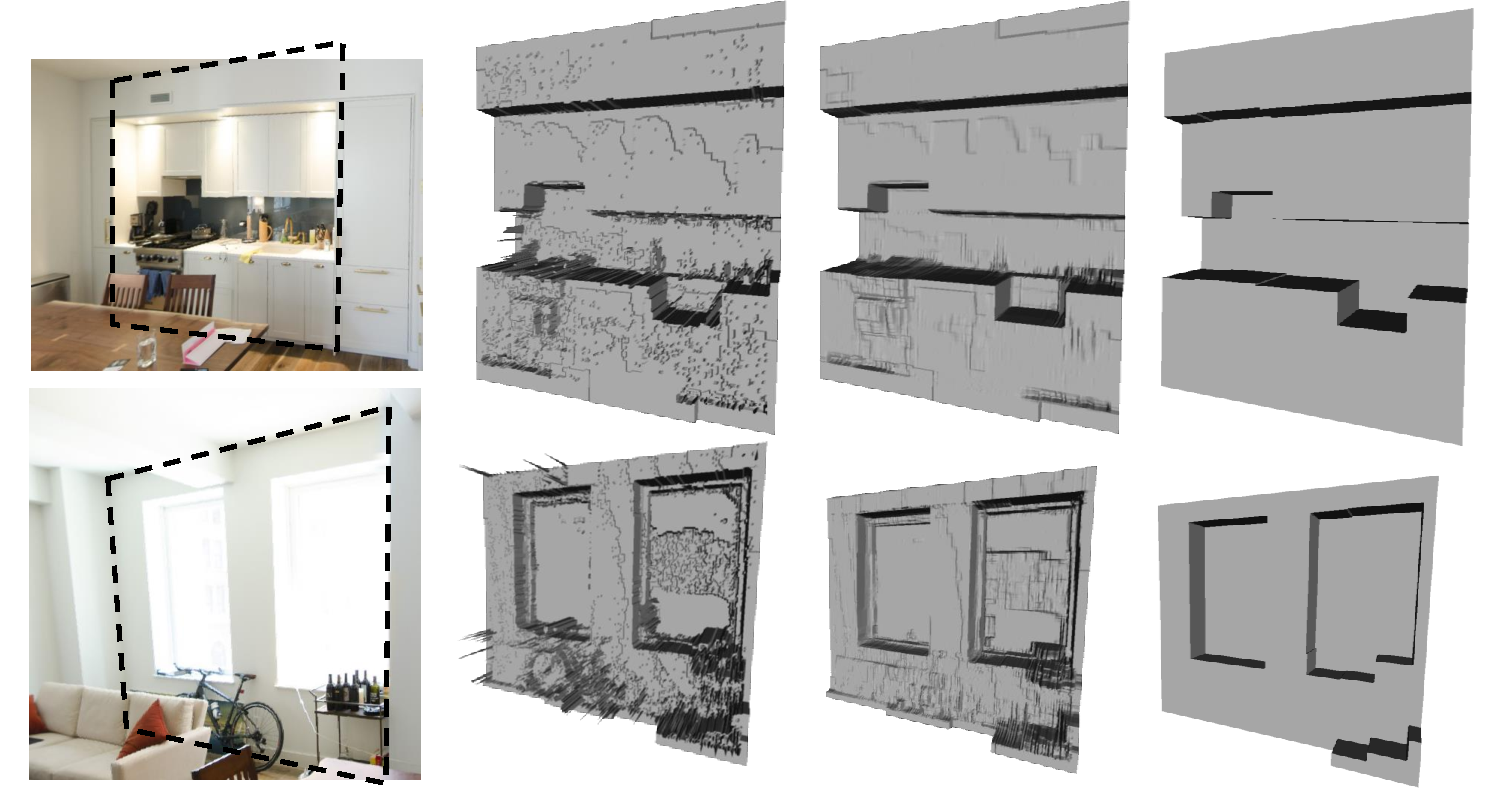
\includegraphics[width=\columnwidth]{../figures/comp_details.pdf}
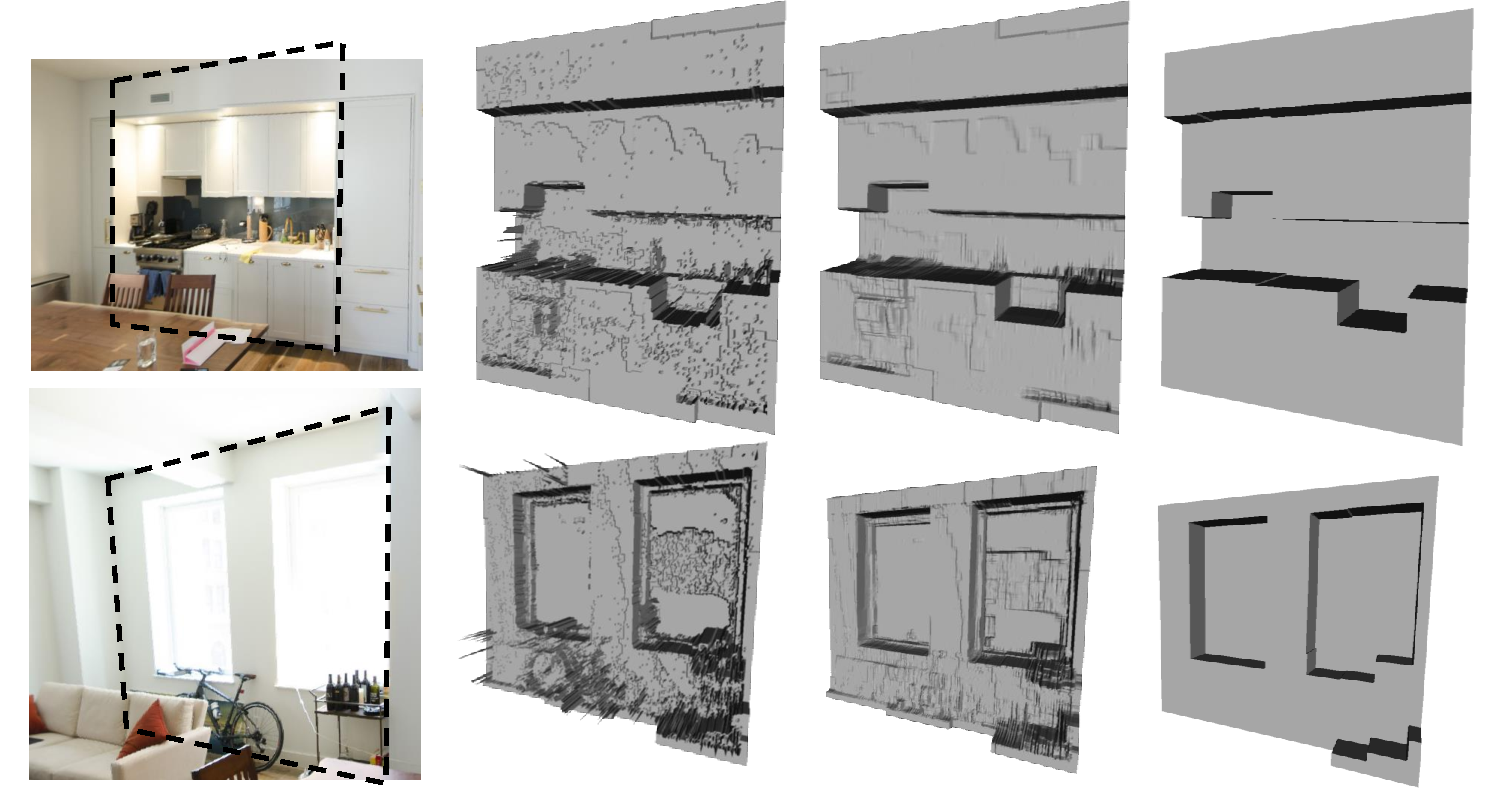
\includegraphics[width=70mm]{../figures/comp_details.pdf} 
\end{center}
\caption{Wall detail reconstruction. From left to right: 1) an image; 2)
 $D_m$ at the initialization; 3) $D_r$ after the RPCA optimization; and
 4) $D_m$ after the MRF (with the label cost) optimization.
%  E xamples of wall/ceiling detail reconstruction. We illustrate
% the surface meshes of the target scene (a), that are reconstructed from
% the offset-maps correspond to (b) $D_0$, (c) $S$, (d) $D$
%in~\Eref{eq:sub1b} and~\Eref{eq:sub2b}.
 } \label{fig:comp_details}
 \vspace{-0.325cm}
\end{figure}
%
The enforcement of piecewise planar ``label boundary'' is a more
challenging problem. We are aware of only one
work~\cite{silberman2014contour}, which effectively enforces this type
of constraint for binary images. However, line segments must be
extracted as the label boundary candidates, and the running time is
exponential in its number.
%We experimented with sparse higher-order MRF~\cite{pushmeet} to enforce
%this constraint, but the optimization became a challenge.
Our key observation is that a piecewise planar ``label boundary'' means
low-rank, where we have an effective optimization tool such as Robust
Principal Component Analysis (RPCA)~\cite{Candes2011} to enforce this
constraint.  
% to enforce low-entropy and low-rank.
%To the best of our knowledge, this work is the first to leveral the
%low-rank structure of the offset-map to enforce geometric regularities.

% The sparsity enforcement
% has been common~\cite{mws,sinha,dave}. However, to the best of our
% knowledge, this work is the first to leverage low-rank structure.

%
% The valid depth range for each pixel is set to be the largest range that
% contains $0$ and fits inside the thresholded 2D free-space region,
% namely $\Psi$ in the room segmentation rule (See
% Fig.~\ref{fig:k-medoids}). The ranges often become too large, and we
% further limit the range to be in $[-1.2\mbox{m}, 0.75\mbox{m}]$ for
% efficiency.
%
Based on our observation, a very compact offset-map is estimated by solving two problems repeatedly:
\begin{eqnarray}
 \min_{D_r}&& \|E\|_1 + \mu_1 \|D_r\|_*\quad s.t.\;\; D_m
 = D_r + E, \nonumber \\
 \min_{D_m}&& \|D_m-D_r\|^2_2 + \mu_2\|\nabla D_m\|_0 + \mu_3Label(D_m) \label{eq:sub2},
\end{eqnarray}
where $\mu_1 = \sqrt{{\rm max}(m,n)}$, $m$, $n$ is the rows and cols of the off-set map. And we set other control parameters as $\mu_2=5.0\times 10^2$ and $\mu_3$ = $10^5$. $D_r$ and $D_m$ denotes the low-rank and low-entropy offset-maps, respectively. This implies that in the first problem, RPCA factorizes the low-entropy matrix into a low-rank structure $D_r$ and a sparse error matrix $E$, and then the number of unique values in the offset-map is reduced in the second problem using $D_r$ as a soft constraint. 

It is worth mentioning that we optimize the second equation as the discrete MRF optimization problem for enforcing the label cost. In this context, the first term in the second problem is a data penalty ensuring the consistency between $D_r$ and $D_m$, the second term is a simple Potts model penalizing the label changes, and the third term is the label cost~\cite{Delong2012} further enforcing the low-entropy structure. 
%Note that RPCA and MRF optimizes different criteria. Therefore, we
%prepare two different offset-map variables, and rely on the constraints
$D_r$ is initialized 
% The only missing piece is the initialization of $D_r$, which is obtained
by a standard MRF with unary and pairwise terms, which reconstructs a raw
offset-map
% by the $\alpha$-expansion algorithm
(See the supplementary material for the definitions of the energy
terms for this step).
%
The iteration converges very quickly in general (2 to 3
iterations). $D_m$ is used as the final offset-map except for $D_r$,
which is low-rank but requires more vertices and polygons (See
Fig.~\ref{fig:comp_details}).


% While MRF takes a cost-volume (\ie, point and free-space evidences) as
% an input, RPCA takes an image (\ie, a depthmap). Therefore, we first use
% a standard MRF with unary and pairwise terms to reconstruct a raw
% offset-map $D_{raw}$ by the $\alpha$-expansion algorithm (See the
% supplementary material for the definitions of the energy terms).  Now,
% the offset-map reconstruction is formulated as the following energy
% minimization problem:
% \begin{eqnarray*}
% \min_{D_{m}, D_{r}, E} &&
%  {|D_{m} - D_{r}|^2_2  +
%  \mu_1 \|\nabla D_{m}\|_0} + \mu_2 {\rm Label}(D_{m}) \nonumber \\
%  +&& \mu_3 \|E\|_1 +\mu_4{\rm Rank}(D_{r}) \quad s.t.\;D_{raw} = D_{r} + E. \nonumber
% \end{eqnarray*}
% We use a coordinate descent and iterate solving $(D_{m})$ and $(D_{r},
% E)$.  Solving for $D_{m}$ corresponds to minimizing the first three
% terms and is exactly the MRF with a label cost. The first term is the
% data-cost, the second term is the Potts model for the pairwise term, and
% the last term is the label cost in the standard definition. Solving for
% $D_{r}$ and $E$ is done by RPCA. Note that RPCA cannot handle the term
% of the form $|D_m-D_r|^2_2$ and only the last two terms and the
% constraint has been enforced. We did not observe a problem in the
% convergence.  Note that MRF is a discrete optimization method and
% $D_{m}$ contains a discrete variable, while $D_{r}$ contains a
% continuous variable. $D_m$ is used as the final offset-map, as $D_r$ 


% In short, the first line corresponds to solving an MRF offset-map
% $D_{m}$ via MRF with a label cost~\cite{Delong2012} for low-entropy, the
% second line corresponds to solving a RPCA offset-map $D_{r}$ via RPCA
% for low-rank, where the first term in the first line makes sure that the
% two depthmaps are close. 
%
% In short, we seek to factorize the raw depthmap $D_{raw}$ into $D$ and
% $E$. $D$ is the final offset-map and must be low-entropy as well as
% low-rank. $E$ is the error matrix and must be sparse.
%$D$ is the final depthmap, where $E$ is the error matrix, which must be 

% where $Label$ is the label cost which is equivalent to the number of
% unique values in the matrix. We put the $\ell_1$-norm minimization term
% of $E$ for quantifying its sparsity of $E$. In addition, we also put the
% $\ell_0$-norm (number of non-zero entries in the matrix) minimization
% term of $\nabla D$ since we are only interested in significant structure
% on the wall and want to remove others.

%
% Our structured indoor scene representation uniquely exports the geometry
% of an entire scene without violoating the rule of manifold-ness, \ie,
% the geometry of the wall and ceiling elements could be represented by a
% plane in a 3-D space whose boundary is smoothly connected to the other
% elements. While those simplified geometry is helpful for visualization
% especially with the texture mapping, however we also observe that there
% are many structures that are functionally inportant for the indoor
% modeling (e.g., window on the wall or spatially varying ceiling
% height). In this section, we reconstruct those {\it details} as childen
% of the walls and ceilings elements.
%
% The main idea is, we recover the $2$-d off-set map of the {\it
% Manhattan-World geometry} instead of reconstructing the geometry in the
% 3-d space. We define the {\it Manhattan-World geometry} as planar
% structures that satisfy that (a) their surface normals are one of
% Manhattan-World directions, (b) they are attached to its parent element
% (e.g., details on the wall, details on the ceil). The reason why we rely
% on the off-set map is mainly two-fold. First, even with any complex
% structures, the manifold-ness of the resultant meshes from an entire
% structured model can be easily preserved. Second, the representation of
% the off-set map, \ie, the matrix, is quite convinent for being optimized
% with the constraint that enforces the Manhattan-World-ness of resultant
% structures.
%
% The challenge of reconstructing the Manhattan-World geometry is how to
% remove the non-Manhattan object that is very close to the element (e.g.,
% the chair in front of the wall), or how can we interpolate the missing
% region that is caused by the sensor missing pixels and those objects.
%



% \begin{equation}
% D_0 = \argmin_{\textbf{l}}{\sum_{p}Cost(p,l) + \lambda \sum_p{\sum_{q\in N(p)}}{Potts(l_p, l_q)}},
% \end{equation}
% On the local coordinate system whose $x-y$ plane is on the element plane
% and the direction of $z$-axis is outgoing direction from the room
% center, we compute the cost as,
% \begin{equation}
% Cost(p,l) = -E^P(p,l)\left(\sum_{k=0}^{l} E^F(p,l)\right),
% \label{eq:costdetail}
% \end{equation}
% where $p$ is the index of a pixel on $x-y$ coordinate and $l \in L$ is
% the candidate label. \Eref{eq:costdetail} quantifies the observation
% that when there is a gap between the outbound geometry and frontal
% object, there should be the freespace-evidence. However, the input point
% cloud is often sparse near the wall and it happens that the ray from the
% viewpoint does not intersect with any points (\ie, the cost for any
% off-set values is zero). For tackling this issue, we simply propagate
% the information from the neighborhood pixels by solving the
% MRF-optimization problem as


% where $Potts$ is the potts penalty that gives zero if two labels are
% same and otherwise one and $D_0$ is the resultant depth map. Since the
% label space is descrete (\ie, the number of the candidate label is the
% depth of the bounding box), we solve this formulation by the Graphcuts
% algorithm.\\




% The reconstruction pipline is three-step, (a) defining the local
% bounding box on the 3-D voxel grid from the parent element, (b)
% intiialize\hang{initialize} the off-set map using the free-space/point
% evidences, (c) reconstruct the Manhattan-World geometry using the intial
% off-set map.

% \noindent\textbf{Local bounding box extraction}

% We firstly define the space of interest that is encoded in the off-set\hang{offset?}
% map.  Practically, we compute the bounding box that is parallel to the
% Manhattan directions whose inbound and outbound range from the parent's
% dominant plane is $\epsilon$. An off-set map is then defined as a depth
% map whose viewpoint is at the inbound boundary of the box and viewing
% direction is outgoing.

% \noindent\textbf{Initializing the off-set map} Once the space of
% interest and the viewpoint of the off-set map are defined, then we
% initialize the off-set map using free-space evidence and
% point-evidence. Intuititatively\hang{Intuitively?} speaking, we cast a ray from the
% viewpoint to the outgoing direction that is perpendicular to the wall,
% and then find the outmost intersection to the surface. More strictly
% speaking, we construct the cost volume whose size is same with the
% bounding box.

% \noindent\textbf{Reconstructing the Manhattan-World geometry}
% The initial off-set map ($D_0$) is generally quite corrupted for mainly two reasons. First, the input free-space evidence and point-evidence are often untrustworthy when there are interior objects in front of the wall. Second, the number of unique values of the initial off-set map ($D_0$) is generally very large, which results in complex surface meshes that give quite low-quality texture-mapped model. 

% For overcoming these issues we rely on the prior knowledge about the man-maid building structure. First, we observe that off-set map contains relatively small number of unique values. Second, we observe that the building details are mostly represented by the planar surfaces whose boundary is clear. This implies that most Manhattan-World geometry on an off-set map is represented by a low-rank matrix. For instance, typical off-set map which has a rectangular on\hang{in?} the middle (\ie, window) could be represented by a rank-$2$ matrix.  

% Under these observation, we can model the initial offset map as a summation of the optimal off-set map  ($D$) and an error matrix ($E$) as $D_0 = D + E. \label{formulation}$, where $D$ is a low-rank matrix whose number of unique values are reasonably small. Even though, we assume the properties of $D$, the decomposition is still ambiguous since we do not have any knowledge about $E$. The standard gaussian assumption on $E$ provides least-squares problem that gives a unique solution, but we found that this formulation is problematic due to the distribution of the error. Since, the input off-set map is highly corrupted by the object that contacts to the wall, the error of off-set map is quite large. Therefore, we model the error matrix $E$ as a sparse matrix whose entries are mostly zero (or very small) and there are a few significant values.



% Since this combinatorial problem is prohibitively complex , we divide the entire problem into subproblems to approximate the solution as 
% \begin{align}
% S &= \argmin_S \|E\|_0 + \mu_1 {\rm rank}(S), \label{eq:sub1} \\
% D &= \argmin_D \|D-S\|^2_2 + \mu_2\|\nabla D\|_0 + \mu_3Label(D) \label{eq:sub2},
% \end{align}
% The main motivation of this problem splitting is we can utilize the recent breakthroughs in convex optimization~\cite{Candes2011} that have shown that~\Eref{eq:sub1} is replaced by the combination of the nuclear norm and $\ell_1$-norm
% minimization problems, and label cost in ~\Eref{eq:sub2} could be minimized when the
% label space is finite and discrete~\cite{Delong2012}. Based on the results, we get following optimization problems to solve:
% \begin{align}
% S &= \argmin_S \|D_0-S\|_1 + \mu_1 \|S\|, \label{eq:sub1b} \\
% D &= \argmin_{D} \sum_{p}\|D(p)-S(p)\|^2_2 \nonumber\\
% 		&+ \mu_2 \sum_p{\sum_{q\in N(p)}}{Potts(D(p), D(q))}+\mu_3\sum_{l\in \mathcal{L}}\delta_L(l).\label{eq:sub2b},
% \end{align}
% %
% %
% %{\small
% %	\begin{fleqn}
% %		\begin{align}
% %		D^{(0)} &= D_0, \nonumber\\
% %		S^{(n+1)} &= \argmin_{S}{|S-D^{(n)}| + \mu_1\|S\|_*}, \label{eq:rpca}\\
% %		D^{(n+1)} &= \argmin_{D} \sum_{p}\|D(p)-S^{(n+1)}(p)\|^2_2 \nonumber\\
% %		&+ \mu_2 \sum_p{\sum_{q\in N(p)}}{Potts(D(p), D(q))}+\mu_3\sum_{l\in \mathcal{L}}\delta_L(l).\label{eq:labelcost}
% %		\end{align}
% %	\end{fleqn}
% %} 
% Here~\Eref{eq:sub1b} is well-known robust princple component analysis
% (RPCA)~\cite{Candes2011} where there already exists multiple solvers
% (\eg, augmenter Lagrangean algorithm) and~\Eref{eq:sub2b} is a
% combination of uncapacitated facility location (UFL) problem and metric
% labeling problems that Delong~\etal have recently proposed the efficient
% solver~\cite{Delong2012}. We should note that the $\ell_0$-norm of the
% gradient of $D$ in~\Eref{eq:original} is replaced by a simple Potts cost
% in~\Eref{eq:sub2b}. 

% Though solving \Eref{eq:sub1b}, \Eref{eq:sub2b} respectively provides good approximation of the solution in~\Eref{eq:original}, MRF result may degenerate the low-rank structure of the depth-map. Therefore, practically we solve~\Eref{eq:sub1b} and~\Eref{eq:sub2b} twice where $D_0$ is replaced by $D_1$ in the second iteration.

% % We should note that the Manhattan geometry reconsturction algorithm is
% % completely same with any elements (\ie, walls, ceilings). Once we an
% % off-set is reconstructed, it is storages as a children ($\textbf{WD},
% % \textbf{CD}$) of the parent node ($\textbf{W}, \textbf{C}$).


\mysubsubsection{Object reconstruction}
The rule takes a room, whose shape has been reconstructed, that is, a
room node with out-going directed edges (pre-condition), then segments
the remaining unexplained 3D points, and generates object nodes
(transformation). Note that a point-cloud is used as the geometric
representation, as the scene visualization is the key application and a
point-based rendering is suitable for incomplete objects rather than a
mesh.
%Object-scale scene understanding and reconstruction has been actively
%studied in the past, where one can simply replace the reconstruction
%algorithm in our framework.

\yasu{given also details}
Given a room node and its extruded 3D model, we first collect 3D points
that are inside the room but not too close to the existing
geometry with a margin of 0.1 times the room height.
% More concretely, we discretize the 3D room space by a voxel grid, so
% that the maximum dimension spans $64$ voxels.  A voxel is marked as $1$,
% if it intersects with the room geometry. After dilating the values in
%the voxel grid twice,
%by a few iterations (2 in our experiments),
A variant of a standard point cloud segmentation algorithm
PCL~\cite{PCL} is used to segment the point-clouds. For better rendering
effects, we remove small objects that contain less than 1000 points, as
well as floating objects whose minimum Z-coordinate is above the room
center.

%where the minor modifications are provided in the supplementary
%material.

% %Further refinements for segmented objects are necessary to get good
% %rendering effect. First,
% we remove small noisy objects which contain
% less than 1000 points, as well as floating objects whose minimum z
% coordinate is greater than half of the room height.

% \mysubsubsection{Room merging} The rule takes two reconstructed room
% nodes if the room connection classifier (explained in detail below)
% identifies the connection type to be ``open'' (pre-condition),  the
% grammar simply removes the two rom nodes, and replace it with a single
% room node (transformation).

% \mysubsubsection{Door addition} The rule takes two wall nodes if the
% room connection classifier identifies the connection type to be ``door''
% (pre-condition). The rule generates a new wall node with a hole at the
% doorway, and adds these two new nodes with a door node in the
% middle. The location of the doorways are also given by the
% classifier. Since the wall node is a simple quad, the geometries of
% these new nodes can be obtained easily.




% In this section, we present a framework to automatically recover the
% structured indoor scene representation from a set of RGB-D point
% cloud. Our framework consists of two main steps: we firstly recover the
% structural elements and their connections and then we reconstruct the
% details of geometry for each structural element. Henceforth we rely on
% the following assumptions:

% \noindent (1) The indoor scene is composed of one-storied rooms. (\ie, the number of floor levels is one).\\
% \noindent (2) Walls are (mostly) parallel to one of the three principal axis of the {\it Manhattan-World coordinate}~\cite{}.


\mysubsubsection{Room connection classification} Pre-conditions of
``door-addition'' and ``room-merging'' depend on the classification of
the room connection types, which are either ``door'', ``merge'', or
``no-connection''. The first and the second classifications are the
pre-conditions of the door-addition and room-merging rules, respectively,
% while no rule will be triggered for no-connection.
This classifier is the key to improve the final room segmentation quality.

Given a pair of rooms, we identify a pair of walls that are parallel,
are within a distance of $1.0$ m vertically (\ie, along the normal), and
have non-zero lateral overlap. For such pair of walls, we compute the
most-likely shape of the door on the walls based on the nearby point and
free-space evidences. More concretely, each wall is discretized into an
array of pixels, whose size is the same as the voxel (\ie,
$0.012$m). The point $P_w(p)$ and free-space $F_w(p)$ evidences on the
wall are obtained by summing $P(v)$ and $F(v)$ along the normal
direction with a margin of 5 voxels, respectively. $P_w$ and $F_w$ are
calculated for each of the two walls, but we know the
correspondence. With abuse of notation, $P_w(p)$ and $F_w(p)$ denote the
sum over the two walls for each pixel $p$.

We want $P_w$ and $F_w$ to be small and large inside the doorway,
respectively. Therefore, the door shape is obtained by finding the
rectangle $\Omega$ that minimizes
\begin{eqnarray}
 \sum_{p\in\Omega} P_w(p)
  - \lambda_1 \sum_{p\in\Omega} F_w(p) + \lambda_2 \{\mbox{area of\
  }\Omega\}.
\end{eqnarray}
The last term is to prefer a smaller rectangle when the solution is
ambiguous due to the lack of evidences. This can be efficiently
computed by using the integral images.
Given the detected rectangle shape and the pair of walls, the connection
type is classified.
%
% The results of the room segmentation step often contains errors, 
% as there is a limit in the 2D analysis from a top-down view.
% Given two adjacent room nodes, we perform this test to determine
% (1) if the two rooms should be connected by a door; (2) if the two rooms
% should be merged; or (3) none of the above, and no action. The decision
% is based on the relationship between the shape of the detected door hole
% and the shape of the wall node, itself.
%
% So far, we extracted multiple room elements ($\textbf{R}$) and the wall
% elements ($\textbf{W}$). However, the number of room elements is not
% always correct due to the over-segmentation by K-medoids clustering. In
% addition, we also need to find the relationship between room elements if
% there is any structural connection. Therefore, in this section, we
% present the framework to analyze the relationship among rooms.
%
%
% Given the label mask presented in the previous section, we find possible
% connections of walls in different rooms by simply detecting the changes
% of labels on 2-D grid. If there is a label change, we assume there could
% be some connections between rooms that are corresponding to those
% labels. However, we do not know in advance\hang{whether?} those connections are
% detected because (a) there is a door between two rooms, (b) two rooms
% should be merged or (c) just simply the connection is
% mis-detected. Therefore we evaluate the type of the connection by
% analyzing the {\it 2-D wall profile}.
%
%
% compute door size. Depending on the relationships, we make
% classifications. For example, ...., the conection is labeled as a door.
% Please see the supplementary material for all the rules.
%
%
% Given a possible connection between between $\textbf{R}_i$ and
% $\textbf{R}_j$, we consider the every pair of wall elements whose parent
% is $\textbf{R}_i$ and $\textbf{R}_j$, respectively. For each wall pair,
% we use the supported 3-D domain for computing two different profiles
% $(PF^F, PF^P)$ computed from the 3-D point evidence $E^P$ and 3-D
% free-space evidence $E^F$ as
% \begin{equation}
% PF^F = \begin{cases}
% 1 & E^F(c_{i,j,\tilde{k}})=1 \;\forall \tilde{k}: -w+k \leq \tilde{k} \leq w+k.\\
% 0 & (otherwise).
% \end{cases}
% \end{equation} 
% \begin{equation}
% PF^P = \sum_{p=-w}^{w}  E^P(c_{i,j,k+p})
% \end{equation} 
% where \{i, j, k\} is the index of cell on the 3-D voxel grid that is on the supported 3-D domain of a wall element, and $w$ is the supported margin (\eg, $5$ in our experiment). We quantify the observation that when there is a connection between two walls, there should not be many points and free-space between them and then solve the following optimization problem to find the connection ($\Omega$) as
% \begin{eqnarray}
% \min_{\Omega \in RectSet} PF^P_1(\Omega) + PF^P_2(\Omega)-\mu_1 (PF^F_1(\Omega) + PF^F_2(\Omega))\nonumber\\
%  - \mu_2 H_\Omega W_\Omega,  
% \end{eqnarray}
% where $RectSet$ is all possible rectangles on the 2-D wall profiles.
%
If the rectangle is too small (the longest dimension is less than $0.6$
m), it is classified as ``no-connection''. The classification between
``door'' and ``merge'' are based on pre-determined thresholds. For
example, if the width and height of the walls are different from those
of the door with a margin, the connection becomes ``door''. Possible
configurations are numerous, and the full classification table is given
in the supplementary material.


% Once extracted the connection, we distinguish connection based on three
% measures, (a) the size of the connection, (b) the margin from the wall
% side and ceiling, (c) the average door size in the same building. First,
% if the size of the connection is smaller than the threshold, we consider
% them as a {\it mis-detected} connection and do not process at all. Then,
% we quantifies the margin between the rectangle's edges and the wall
% edges and ceiling and categorize the connection as either of "door" or
% "merge" based on the classification table~\Fref{fig:dooranalysis}. Since
% this table is heuristic and not always perfect, we also consider the
% statistical distribution of the width of connection. Since the door is
% designed for human ant its size is not largely different in the same
% building, we assume that when the width of the rectangle is
% significantly bigger than the other "door" rectangles, we conclude the
% door is mis-classified and changed the label into the "merge". Strictly
% speaking, we compute the minimum and the standard deviation of the
% rectangular widths and when the width of a rectangular that is
% classified as "door" is more than a minimum plus the twice of the
% standard deviation, we change the label into the "merge".



%Once, the connection is classified as the "door", the corners of the
%rectangle are storaged in the \textbf{D}.Corner1 and \textbf{D}.Corner2
%and the connection is classifed as "merge", we merge two room elements
%as shown in the next section.



% \begin{figure}[t]
% 	\begin{center}
% 		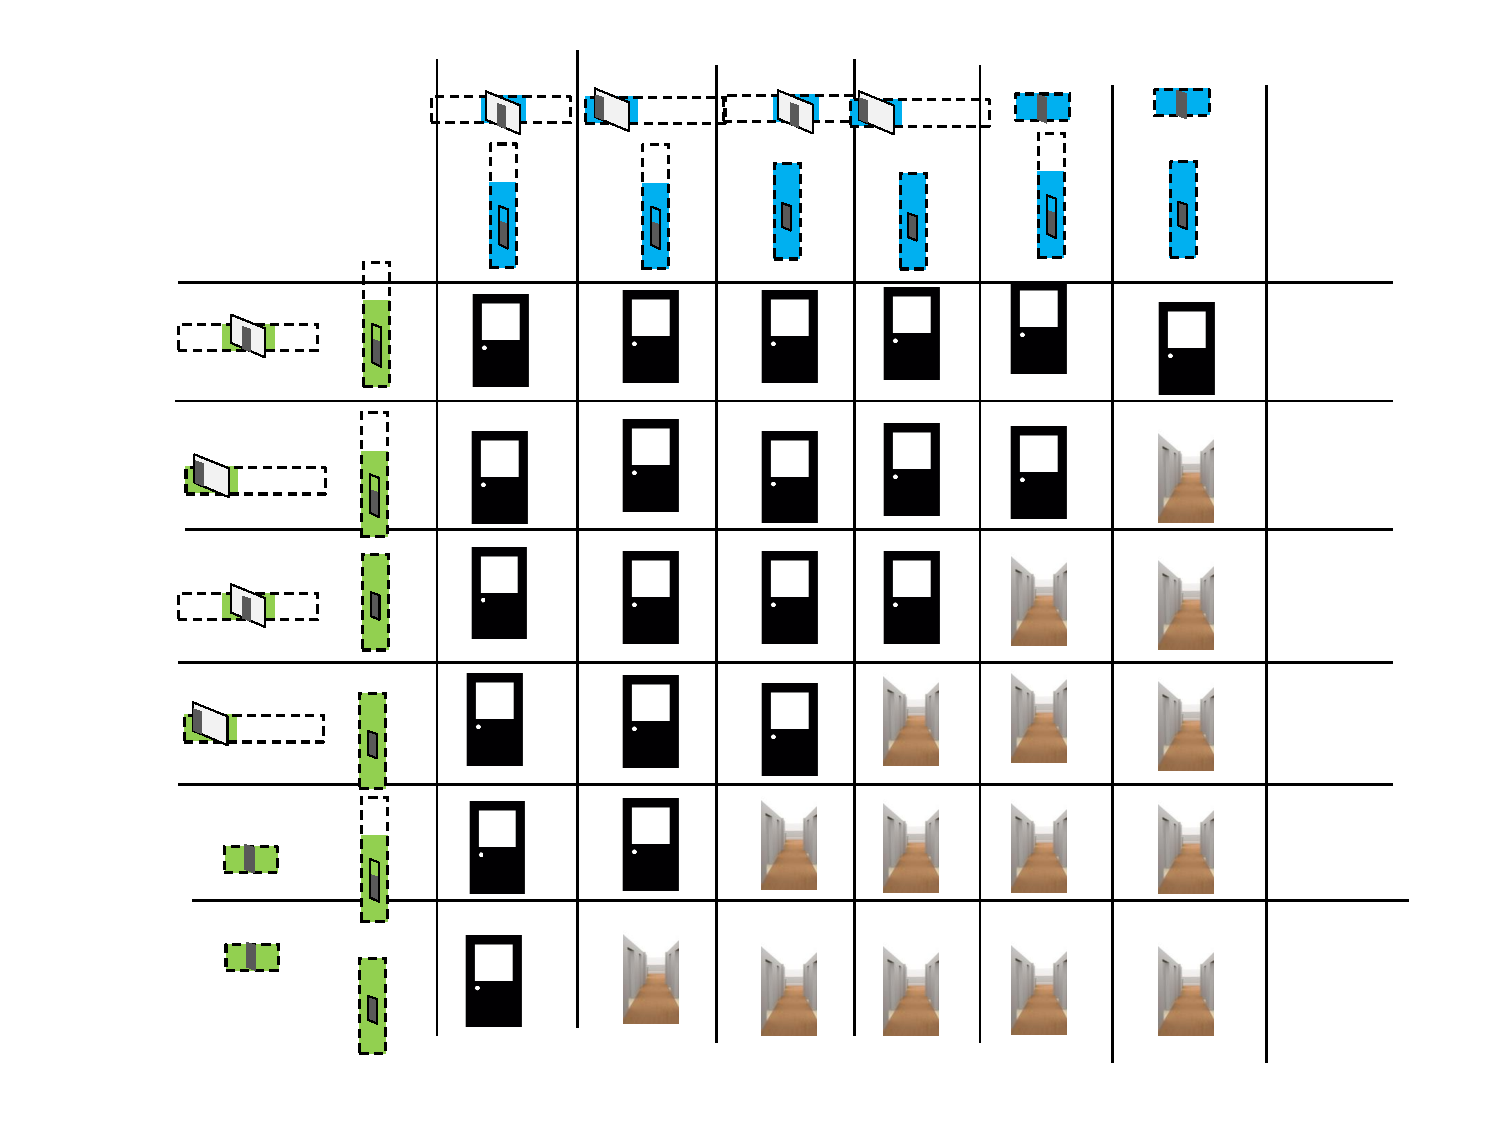
\includegraphics[width=85mm]{../figures/dooranalysis}
% 	\end{center}
% 	\caption{Judging criteria of the wall profile analysis.}
% 	\label{fig:dooranalysis}
% \end{figure}


%These point-evidence and free-space evidence are used in many steps in our entire framework, and generally these evidences must be dense. Therefore we perform 2D morphological closing operation on the both $\tilde{E^P} and \tilde{E^F}$ (using disk kernel whose radius is mostly one or two).
% \subsection{Preliminaries}
% In this section, we describe the elements that define the structured indoor scene representation. \\
% \begin{table}
% \caption{Symbols in our framework }
% \begin{tabularx}{85mm}{|c|X|}
% \hline $P$ & Input point cloud $(x,y,z,n_x,n_y,n_z,r,g,b)$ \\
% \hline $P^W$ & Subset of $P$ whose normal is pointing at one of $\pm X,\pm Y$ \\
% \hline $E^F$ &  3D free-space evidence computed from $P$\\
% \hline $E^P$ &  3D point evidence computed from $P$\\ 
% \hline $E^W$ &  3D wall evidence computed from $P^W$\\ 
% \hline $\tilde{E}^F$ & 2D free-space evidence computed from $E^F$\\ 
% \hline $\tilde{E}^P$ & 2D point evidence computed from $E^P$\\ 
% \hline $\tilde{E}^W$ & 2D wall evidence computed from $E^W$\\ 
% \hline $\Omega$ & Core free-space evidence on 2D voxel grids\\
% \hline $U$ & Pixel index of unexplained free-space on 2D voxel grid\\
% \hline $A$ & Aisle connection matrix that indicates $i$-th room and $j$-th room must be merged when $A_{i,j}=1$ \\
% \hline
% \end{tabularx}  
% \end{table}









% %\subsection{Room, Wall, Door Elements Reconstruction}
% %%%%%%%%%%%%%%%%%%%%%%%%%%%%%%%%%%%%%%%%%%%%%%%%%%%%%%%%%
% \begin{algorithm}[t]
% \caption{Room, Wall, Door Elements Reconstruction}\label{algo:segmentation}
% \begin{algorithmic}[t]
% \STATE \textbf{Input}: 3D Free-space evidence $E^F$, 2D Freespace evidence $\tilde{E}^F$, 3D Point evidence $E^P$, 2D Point evidence $\tilde{E}^P$
% \STATE \textbf{Output}: Room elements $\textbf{R}$, Wall elements $\textbf{W}$, Door elements $\textbf{D}$
% \STATE $\hat{\textbf{R}} \leftarrow {\rm KmedoidsSegmentation}(\hat{E^F})$
% \STATE $\Omega = {\rm CoreExtraction}(\hat{\textbf{R}})$ 
% \STATE $\hat{\textbf{W}} = {\rm PathReconstruction}(\tilde{E}^F, \tilde{E}_W^P, \Omega, \hat{\textbf{R}})$
% \STATE $U \leftarrow {\rm FindUnexplainedRegion}(\tilde{E}^F,\tilde{E}^P,\textbf{W},\hat{\textbf{R}})$
% \WHILE{$U\neq \emptyset$}
% \STATE $\hat{\textbf{R}}\leftarrow \hat{\textbf{R}}\bigcup U$
% \STATE $C = {\rm CoreExtraction}(U)$ 
% \STATE $\hat{\textbf{W}}\leftarrow \hat{\textbf{W}}\bigcup {\rm PathReconstruction}(\tilde{E}^F, \tilde{E}_W^P, C, U)$
% \STATE $U \leftarrow {\rm FindUnexplainedRegion}(\tilde{E}^F, \tilde{E}^P,\hat{\textbf{W}},\hat{\textbf{R}})$
% \ENDWHILE
% \STATE $[\textbf{D}, A]={\rm WallProfileAnalysis}(E^F, E^P, \hat{\textbf{W}}, \hat{\textbf{R}})$
% \WHILE{$A=\emptyset$}
% \STATE [$\hat{\textbf{W}}, \hat{\textbf{R}}]\leftarrow {\rm MergeRooms}(\hat{\textbf{W}}, \hat{\textbf{R}}, A, \tilde{E}^F, \tilde{E}^P)$
% \STATE $[\hat{\textbf{D}}, A]={\rm WallProfileAnalysis}(E^F, E^P, \hat{\textbf{W}}, \hat{\textbf{R}})$
% \ENDWHILE
% \STATE $\textbf{R} \leftarrow \hat{\textbf{R}},\; \textbf{W} \leftarrow \hat{\textbf{W}},\; \textbf{D} \leftarrow \hat{\textbf{D}}$
% \end{algorithmic}
%  \yasu{Convert this to a bubble-flow-chart with arrows.}
% \end{algorithm}
% %%%%%%%%%%%%%%%%%%%%%%%%%%%%%%%%%%%%%%%%%%%%%%%%%%%%%%%%%%%%%%%%%%%%%%%%%%%%%%
% Among the structual elements, the room, wall and door elements form the horizontal structure of an indoor scene while the floor and ceiling describes the vertical relationship. Therefore, in this section we present the framework to reconstruct only room, wall, door elements on the 2D domain and then we reconstruct the ceiling and floor in the next section. 

% We solve the problem by mainly three steps. (1) we perform the room
% segmentation algorithm to get the correct number of room elements and
% then assign a sub-set of the input point cloud to each room element, (2)
% we reconstruct the wall elements from the point cloud assigend to the
% parent room element, (3) we extract the door connection between walls of
% two different rooms and connect the wall nodes via extracted door
% element. In practice, we iteratively solve from (1) to (3) unitl
% convergence to refine the structured reconstruction gradually as shown
% in~\Aref{algo:segmentation}. In the rest of this section, we detail the
% algorithm.




% \noindent \textbf{Iterative updating the room, wall, door elements}

% Once the room elements are updated, we also compute the connection
% between existing rooms and newly merged room.  If new "open" connection
% is extracted, we iteratively perform the merging until there is no
% "open" connection. The entire algorithm is shown in~\Aref{algo:}



